
\chapter{Implementation details}
\label{implementation}
% Here we describe some of the important implementation details.

DECS has been implemented in the C++ programming language and the source code is available at \url{http://decs.googlecode.com/} licensed under the GNU General Public License version 2.
The DECS software suite consists of several parts:
\begin{description}
	\item[libdecs]
		This static library contains all the essential parts of DECS like the DLX algorithm, the sparse boolean matrix representation code and the file input/output functionality.
	\item[dance]
		The dance command line program can solve exact covers stored in the DECS file format.
		It can also display various information about the content of a DECS file.
	\item[bdance]
		The bdance program is integrated with the BOINC framework.
		This is the program that any BOINC client connected to the DECS project will download and use.
		It simply reads from the file in.decs, solves the exact cover and writes the solutions to the out.decs file.
	\item[degen]
		The DECS matrix generator is a command line program which can build exact cover matrices and save them in the DECS file format.
		It can also do reverse transforms and analyze DECS result files from previous computations.
		It relies on a set of libraries to do forward and reverse transforms on the specific type of problem.
		Currently the only library available is for the $n$-queens problem.
\end{description}



\section{Architecture}

The DECS system architecture is layer based as shown in Figure \ref{fig:architecture}.
The application layer is where external applications produce exact cover problems and where the final solutions end up.
The transformation layer is where the degen program and its libraries operate.
The generalization step is when degen receives a problem, turns it into an exact cover problem and outputs the matrix in the DECS file format.
This file is then handed to libdecs where the DLX parallel recursive splitter (Algorithm \ref{alg:psearch}) produces a number of work units.
Each of the work units are handed to the BOINC system, which makes sure that they are available for clients connected to the BOINC server provided by DECS.
When a client receives a work unit it runs the DLX algorithm (Algorithm \ref{alg:isearch}) to find all the solutions.
The client then sends the solutions back the the BOINC server where they are verified for correctness and stored until the solutions to all the related work units has been received.
BOINC then hands the solutions back to libdecs which reads and analyzes the solution files and merges them into a single file.
Finally it passes the resulting file to the degen program which runs a reverse transform on the solutions.
It then writes the final results in whatever format the application needs.

\begin{figure}[htbp]
	\centering 
	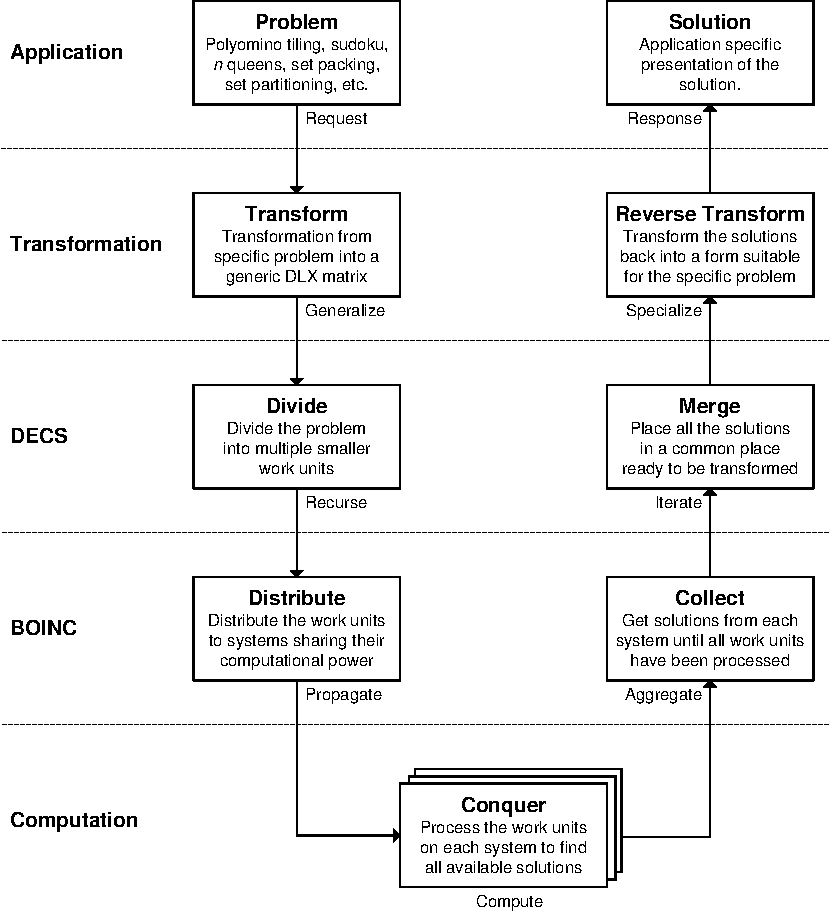
\includegraphics[width=0.85\textwidth]{architecture.pdf}
	\caption{Generic Distributed Exact Cover Solver system architecture}
	\label{fig:architecture}
\end{figure}



%\section{BOINC}

% TODO: Important - Write more about BOINC.
%\subsection{Architecture}

%Components of a BOINC server
%\begin{itemize}
%	\item Feeder
%	\item Transitioner
%	\item File deleter
%	\item Application
%	\item Work generator
%	\item Validator
%	\item Assimilator
%\end{itemize}

% To keep track of the different files and work units BOINC renames them and keeps track of them by storing their names in a database.



\section{Transforms}
\label{transforms}

To turn a specific problem into an exact cover problem an algorithm is needed that understands that specific problem.
This algorithm then turns the problem into an exact cover matrix which can be solved by the DLX algorithm.
When the solutions to the matrix has been found they need to be translated back (reverse transform) into the domain of the original problem so that it is possible to understand the end result.
The degen program makes use of a set of libraries to accomplish these two task.


\subsection{\texorpdfstring{$n$}{n}-queens}
\label{queens_trans}

The $n$-queens problem has been described in detail in Section \ref{intro_queens} along with an example in Section \ref{general_exact_cover}.
It was originally proposed by the chess player Max Bezzel in 1848.
Since that time many people has made an effort to find the number of solutions for steadily increasing values of $n$.
The next unsolved puzzle is for $n = 26$ which is expected to have somewhere around $2 \times 10^{16}$ solutions.
Trying to parallelize the $n$-queens problem is nothing new.
As early as 1989 Bruce Abramson and Moti Yung presented a divide and conquer algorithm in \cite{Abramson89} which in principle could be used to do parallel processing.
A Danish bachelor project from the spring of 2007 \cite{queens-mig} tried to solve the problem for $n=26$ on the MiG \cite{mig} Grid computing platform.
One of the most promising projects lately is the BOINC based NQueens@Home \cite{nqueensathome} project.
About 13 years of CPU time has been registered by the project after running for only 3 months.

Algorithm \ref{alg:nqeens-cover} shows how the $n$-queens transform takes place.
The parameter $A$ is a matrix (or two dimmensional array) with all elements set to zero, $i \times j$ rows, $2n$ primary columns and $4n - 6$ secondary columns (for the two diagonals).
The elements in $A$ are accessed by $A[i,j]$ where $i$ is the row, $j$ is the column and both values start at zero.
Each iteration through the inner loop generates one row in the matrix for each file on the chessboard.
The outer loop steps through all the ranks on the board and by multiplying the number of ranks and files we get $n^2$ rows in the final matrix.
Each of these rows represents a unique placement of a queen on the chessboard.
The algorithm is made a bit complex by the calculation of each of the two diagonals.
At the end of the algorithm the matrix $A$ can be saved to file and made ready for further processing.

\begin{algorithm}[H]
	\caption{Transforming $n$-queens into the exact cover matrix $A$.}
	\label{alg:nqeens-cover}
%	\algsetup{indent=5em}
	\begin{distribalgo}[1]
		\PROCEDURE{queens-tf($n$, $A$)}
			\FOR{$i \leftarrow 0$ \textbf{to} $n - 1$}
				\FOR{$j \leftarrow 0$ \textbf{to} $n - 1$}
					\STATE $row \leftarrow i \times j$
					\STATE $A[row,i] \leftarrow 1$  \COMMENT{The rank}
					\STATE $A[row,j+n] \leftarrow 1$  \COMMENT{The file}
					\STATE $d_1 \leftarrow i + j$  \COMMENT{The first diagonal}
					\IF{$d_1 \neq 0$ and $d_1 \neq 2n - 2$}
						\IF{$d_1 < 2n - 2$}
							\STATE $A[row,d_1 + 2n - 1] \leftarrow 1$
						\ELSE
							\STATE $A[row,d_1 + 2n - 2] \leftarrow 1$
						\ENDIF
					\ENDIF
					\STATE $d_2 \leftarrow n - i + j - 1$  \COMMENT{The second diagonal}
					\IF{$d_2 \neq 0$ and $d_2 \neq 2n - 2$}
						\IF{$d_2 < 2n - 2$}
							\STATE $A[row,d_2 + 4n - 4] \leftarrow 1$
						\ELSE
							\STATE $A[row,d_2 + 4n - 5] \leftarrow 1$
						\ENDIF
					\ENDIF
				\ENDFOR
			\ENDFOR
		\ENDPROC
	\end{distribalgo}
\end{algorithm}

Algorithm \ref{alg:nqeens-reverse} shows how to place the queens on the $8 \times 8$ chessboard when a solution has been found.
The input parameters to the algorithms is the solution $S$, which is a set of row numbers, and the number of queens $n$.
It uses zero based row numbers and provides zero based rank and file values as a result.
\begin{algorithm}[H]
	\caption{Reverse transforming $n$-queens to chessboard placements.}
	\label{alg:nqeens-reverse}
%	\algsetup{indent=5em}
	\begin{distribalgo}[1]
		\PROCEDURE{queens-rtf($S, n$)}
			\FOREACH{row $i$ in $S$}
				\STATE $f \leftarrow i \bmod n$
				\STATE $r \leftarrow (i - f) / n$
				\STATE Place a queen at file $f$ and rank $r$.
			\ENDFOR
			\STATE Show chessboard.
		\ENDPROC
	\end{distribalgo}
\end{algorithm}

\begin{example}
Using the dance program to solve the 8-queens problem gives us a list of 92 solutions like this
\begin{verbatim}
$ dance --verbose examples/queens8.decs
[...]
Solution: 3 15 20 26 49 61 32 46
[...]
Search complete

Number of solutions: 92
\end{verbatim}
The solutions contains the row numbers from the matrix and not the entire content of the rows.
The row numbers given in the output are zero based.
Using the reverse transform algorithm above with $S = \{3, 15, 20, 26, 49, 61, 32, 46\}$ and $n = 8$ the queens are placed on the chessboard where they belong.
Working though the list of rows reveals the same chessboard as shown in Figure \ref{fig:8queens}.
\end{example}




%\subsection{Polyominoes}
%\label{poly_trans}

%Solomon W. Golomb practically invented the concept of polyominoes and made it widely available in his book \cite{Polyominoes}.


%\subsection{Latin square}
%\label{latin_trans}

%\cite{Colbourn04}
% Application of Exact Cover to Solving the Latin Square Puzzle
% -- http://www.imtek.de/simulation//mathematica/IMSweb/imsTOC/Game%20Theory/ExactCoverDocu.html

%Latin square puzzles - Special types of Latin squares can be used as error correcting codes for power line communication (sending radio signals over electric power lines) \cite{Colbourn04}


%\subsection{Sudoku}
%\label{sudoku_trans}

% Sudoku (special case of Latin squares)
%Granted Sudoku 



\section{File format}

In order to store and transfer a DLX problem matrix efficiently a file format had to be defined for this specific purpose.


\subsection{Byte ordering}

Several challenges arise when defining a file format, but one of the most common is that of byte ordering.
Different platforms use different byte ordering, meaning that the order of the bytes in variables bigger than 1 byte may differ from one system to another.

Byte ordering deals with how the bytes for individual variables are ordered in memory.
For a 1 byte large variable the byte ordering is irrelevant as it is only possible to order that single byte one way.
For variables larger that 1 byte the order the bytes appear in when read from and written to memory follow one of the two major conventions: big-endian or little-endian.

Big-endian stores the most significant byte (MSB) first and the least significant byte (LSB) last while little-endian does it the other way around.
In Table \ref{tab:endian} we can see that the value 0x7E, when stored in a single byte of memory, is represented in the same way for both types of byte ordering.
However, when the same value is stored in 2 bytes of memory the difference is clearly visible.

\begin{table}[htbp]
	\centering
	\begin{tabular}{|l||l|l||l|}
		\hline
		\bf Byte order & \bf 1 byte & \bf 2 bytes & \bf 4 bytes \\ \hline
		Big-endian    & 7E & 00 7E & 12 34 56 78 \\ \hline
		Little-endian & 7E & 7E 00 & 78 56 34 12 \\ \hline
	\end{tabular}
	\caption{Difference in representation between little and big endian when storing the value 0x7E and 0x12345678.}
	\label{tab:endian}
\end{table}

In order to achieve portability between different processor and operating system platforms one has to choose either big-endian, little-endian or a bit to indicate the byte ordering used in the file.
It is also possible to use a endian-neutral format like ASCII text or the External Data Representation (XDR) \cite{RFC4506} standard.
To make the file format consistent across platforms little-endian was chosen.
Following the recommendations of Intel's Endianness White Paper \cite{intel-endian} the proper byte swapping methods for big-endian systems has been implemented.


\subsection{Storing sparse boolean matrices}

The storage format for the sparse boolean problem matrix has been designed for fast and efficient reading.
All values are unsigned integers unless explicitly stated otherwise.
For more information on how the matrix data structure is constructed when it is read from file, see Section \ref{matrix_construction}.

The main file header format is made as simple as possible to allow future extensions to be made without breaking backwards compatibility.
In every DECS formatted file the 8 first bytes of the file are occupied by the main header as shown in Table \ref{tab:header-main} and Figure \ref{fig:header-main}.
Currently only the first byte of the version field is used.
In a future versions both bytes in the version field are planned to be ASCII characters so that a separate ASCII format can be defined.
The type field indicates how the data following the header will look like.
When the ASCII format is defined it will probably use the two ASCII characters ``M'' and ``R'' to indicate the type of file.

%The version field indicates the lowest possible file format version implemented which will be able to read this version of the file.
%This means that if the file format version implemented in a program is lower than the compat field it will not be able to read and process it correctly.

\begin{table}[htbp]
	\centering
	\begin{tabular}{|r|r|p{3.1in}|}
		\hline
		\bf Offset & \bf Length & \bf Description \\ \hline
		0  & 4 & \texttt{fileid} - File type ID: ``DECS'' \\ \hline
		4  & 2 & \texttt{version} - File format version. \\ \hline
		6  & 1 & \texttt{type} - 0 for exact cover matrix and 1 for results. Other values are currently unused. \\ \hline
		7  & 1 & \texttt{reserved} - Reserved for future use. \\ \hline
	\end{tabular}
	\caption{Main file header format. Offset and length in bytes.}
	\label{tab:header-main}
\end{table}

\begin{figure}[htbp]
	\centering
	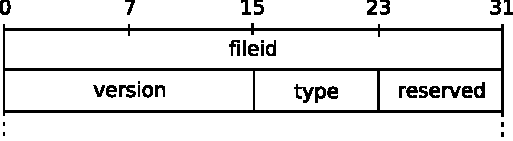
\includegraphics[width=0.57\textwidth]{header-main.pdf}
	\caption{Main file header format structure}
	\label{fig:header-main}
\end{figure}


\subsubsection{Matrix file format}

When the type field in the main header is 0 then the file contains an exact cover matrix.
It also means that the 40 bytes following the main header is part of the matrix file format header.
The full structure of the matrix header is shown Table \ref{tab:header-matrix} and Figure \ref{fig:header-matrix}.

The DLX algorithm does not use the column and row names that \texttt{name\_off} points to or the problem ID and the problem specific information.
This information can be used by the BOINC client to display graphical information during the computation.
For example it can use the problem ID to identify the correct transform, and when the DLX algorithm finds a solution it can run the reverse transform and display the solution graphically.
As an example the $n$-queens problem could update the screen every 5 second with the last solution found along with the total number of solutions found at that point.
BOINC has built-in support for OpenGL rendering and the solutions could be displayed as part of a special BOINC screen saver.
The structure of the problem information is up to the developers of the problem specific library to determine.
The only requirement is that the first 4 bytes must contain the size of the data (including the value itself) as an unsigned 32-bit integer.

One special note should be made of the bit flags at offset 44.
The least significant bit (LSB) in the bit flag value is the ``conserve bandwidth`` flag.
When the conserve bandwidth flag is set only the number of solutions should be stored in the DECS result file when the problem has been solved.
If the conserve bandwidth flag is not set then every single solution is stored in the result file.
This setting can be overridden by the presence of a special command line argument.
The rest of the bits are yet to be assigned a value and meaning.

\begin{table}[htbp]
	\centering
	\begin{tabular}{|r|r|p{3.2in}|}
		\hline
		\bf Offset & \bf Length & \bf Description \\ \hline
		8  & 4 & \texttt{cols\_num} - Number of columns $> 1$. \\ \hline
		12 & 4 & \texttt{rows\_num} - Number of rows $> 1$. \\ \hline
		16 & 4 & \texttt{elems\_num} - Number of non-zero values in the matrix $> 1$. \\ \hline
		20 & 4 & \texttt{elems\_off} - Byte offset to the matrix element entries. Should never be 0. \\ \hline
		24 & 4 & \texttt{secol\_off} - Byte offset to the secondary column list. 0 if unavailable. \\ \hline
		28 & 4 & \texttt{init\_off} -  Byte offset to the initialization vector. 0 if unavailable. \\ \hline
		32 & 4 & \texttt{name\_off} - Byte offset to the column and row name list. 0 if unavailable. \\ \hline
		36 & 4 & \texttt{prob\_id} - Problem ID. Each problem type has a unique ID so that the correct transform can be chosen and the problem specific information can be decoded. \\ \hline
		40 & 4 & \texttt{prob\_off} - Byte offset to problem specific information. 0 if unavailable. \\ \hline
		44 & 4 & \texttt{flags} - Bit flags for various purposes. \\ \hline
	\end{tabular}
	\caption{Matrix file header format. Offset and length in bytes.}
	\label{tab:header-matrix}
\end{table}

\begin{figure}[htbp]
	\centering
	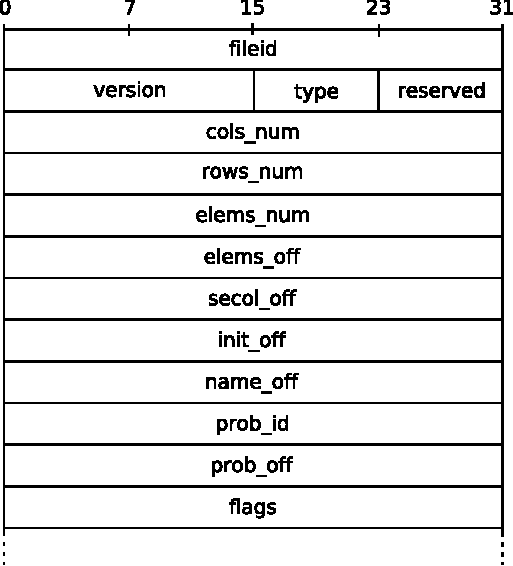
\includegraphics[width=0.57\textwidth]{header-matrix.pdf}
	\caption{Matrix file header format structure including the main header}
	\label{fig:header-matrix}
\end{figure}


\subsubsection{Result file format}

If the type field in the main header is 1 then the file contains the results of an exact cover problem.
The size of the result header is 16 bytes as shown in Table \ref{tab:header-result} and Figure \ref{fig:header-result}.

When the DLX algorithm has solved an exact cover problem it stores the results in a file using the result file format.
If the conserve bandwidth flag is set in the matrix file then \texttt{results\_off} will be zero.
This indicates that no solutions are stored in the file.

\begin{table}[htbp]
	\centering
	\begin{tabular}{|r|r|p{3.2in}|}
		\hline
		\bf Offset & \bf Length & \bf Description \\ \hline
		8  & 4 & \texttt{results\_num} - Number of results. \\ \hline
		12 & 4 & \texttt{results\_off} - Byte offset to the list of solutions. 0 if unavailable. \\ \hline
		16 & 4 & \texttt{prob\_id} - Problem type ID. Each problem type has a unique ID so that the correct transform can be chosen and the problem specific information can be decoded. \\ \hline
		20 & 4 & \texttt{prob\_off} - Byte offset to problem specific information. 0 if unavailable. \\ \hline
	\end{tabular}
	\caption{Result file header format. Offset and length in bytes.}
	\label{tab:header-result}
\end{table}

\begin{figure}[htbp]
	\centering
	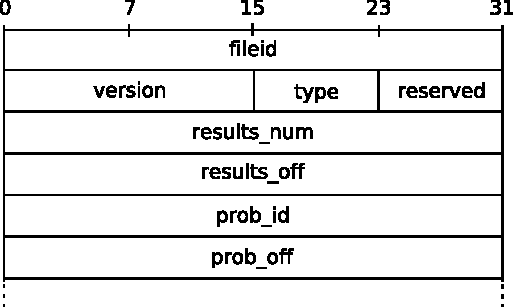
\includegraphics[width=0.57\textwidth]{header-result.pdf}
	\caption{Result file header format structure including the main header}
	\label{fig:header-result}
\end{figure}



The structure of the data pointed to by many of the byte offsets are simple lists that consists of unsigned 32-bit integers.
This format is used by the solution list (\texttt{results\_off}), matrix element list (\texttt{elems\_off}), secondary column list (\texttt{secol\_off}) and the initialization vector list (\texttt{init\_off}).
The first value $n$ is the size of the list indicating how many unsigned 32-bit integers it contains.
Reading the following $n$ values ($4n$ bytes) provides all the elements of the list.
The solution list and matrix element list are actually a sequence of lists where each list represents one solution (set of rows) or one row in the matrix (set of columns numbers for elements with non-zero values).
By using the value read from the respective header fields \texttt{results\_num} or \texttt{rows\_num} the correct number of lists can be obtained from the file.



\section{libdecs}


\subsection{Modes of operation}

DECS has two basic modes of operation regarding how it handles the return values in the system.
In the first mode each client will store and forward all the solutions it finds back to the BOINC server.
This provides the calling application with the full set of solutions so that it can run a detailed analysis on them or save them for later use.
For problems which generates a very large number of solutions this approach can cause a huge strain on the system.
The storage and bandwidth capacities of the computing nodes and the BOINC server would quickly become a bottleneck if there are too many solutions.
In extreme cases it might even cause some of the solutions to never be returned because the system is unable to handle the load.
A policy of not accepting overly large problem matrices could be implemented to prevent this problem.

The second mode of operation will discard the actual results, but instead keep a count on how many solutions has been found.
When a matrix has been solved it only returns the value holding the number of solutions to the server.
This drastically reduces the bandwidth and storage requirements for the clients and servers, but it also makes it impossible to analyze the final solutions.
This is the default mode used by the $n$-queens library because there we are usually not interested individual solutions.
Instead we only want to know the total number of solutions.

A possible extension to this would be to add other return values than the number of solutions.
Each solution the DLX algorithm finds could be further analyzed so that other aspects of the solutions could be returned.

%The main purpose of libdlx is to parse a file with the problem matrix and to apply the DLX algorithm in order to solve it.
%The theory behind the DLX algorithm has been covered in Chapter \ref{dancing_links}.
%Here we will look at the external interface to libdlx and some of its internals.


\subsection{Building the boolean matrix}
\label{matrix_construction}

Before the DLX algorithm can be started the matrix needs to be read from a file and the data structures must be initialized.
Each non-zero element in the matrix is a quad-linked node in a circular quad-linked structure.

To construct the matrix data structure we have some special column objects.
Before the nodes are added a root node is created which is the basis for the entire structure.
To the right of the root node all the column header nodes are added in the order of increasing column indices.
Algorithm~\ref{alg:columns} shows how the circular doubly-linked column list is created.
It starts by creating the root node $R$ onto which all the column nodes are attached.
Take special note of how the secondary column objects are linking to themselves on line 10 and 11.

\begin{algorithm}[H]
	\caption{Create the circular doubly-linked list of columns.}
	\label{alg:columns}
%	\algsetup{indent=5em}
	\begin{distribalgo}[1]
		\STATE $R \leftarrow$ new column object
		\STATE $T \leftarrow R$
		\FOR{$i \leftarrow 1$ \textbf{to} the value of the \texttt{cols\_num} field}
			\STATE $C \leftarrow$ new column object with index $i$
			\IF{column $i$ is a primary column}
				\STATE $C.left \leftarrow T$  \COMMENT{Add primary column header}
				\STATE $T.right \leftarrow C$
				\STATE $T \leftarrow C$
			\ELSE
				\STATE $C.left \leftarrow C$  \COMMENT{Add secondary column header}
				\STATE $C.right \leftarrow C$
			\ENDIF
			\STATE $H[i] \leftarrow C$
		\ENDFOR
		\STATE $R.left \leftarrow T$
		\STATE $T.right \leftarrow R$
	\end{distribalgo}
\end{algorithm}

To initialize the data structure the nodes must be added row by row by reading them from the left to the right side.
The algorithm starts with the top row and works its way down to the bottom.
It also makes use of the column header array $H$ which was initialized in Algorithm \ref{alg:columns}.

\begin{algorithm}[H]
	\caption{Create the circular quad-linked node structure.}
	\label{alg:nodes}
	\begin{distribalgo}[1]
		\FOR{$i \leftarrow 1$ \textbf{to} the value of the \texttt{rows\_num} field}
			\FOREACH{column index $j$ in row $i$}
				\STATE $N \leftarrow$ new node object with row index $i$
				\STATE $C \leftarrow H[j]$
				\STATE $N.column \leftarrow C$
				\STATE $C.size \leftarrow C.size + 1$  \COMMENT{Increment column size}
				\STATE $N.up \leftarrow C.up$  \COMMENT{Add element to column list}
				\STATE $N.down \leftarrow C$
				\STATE $C.up.down \leftarrow N$
				\STATE $C.up \leftarrow N$
				\IF{$T$ is set}
					\STATE $N.left \leftarrow T$  \COMMENT{Add element to row list}
					\STATE $N.right \leftarrow T.right$
					\STATE $T.right.left \leftarrow N$
					\STATE $T.right \leftarrow N$
				\ELSE
					\STATE $N.left \leftarrow N$  \COMMENT{First node in a row}
					\STATE $N.right \leftarrow N$
				\ENDIF
				\STATE $T \leftarrow N$
			\ENDFOR
			\STATE Unset $T$
		\ENDFOR
	\end{distribalgo}
\end{algorithm}


